\documentclass[10pt,a4paper]{article}
\usepackage[english]{babel}
\usepackage[utf8]{inputenc}
\usepackage{amsmath}
\usepackage{amsfonts}
\usepackage{amssymb}
\usepackage{graphicx}
\usepackage{float}
\usepackage{caption}

%link to documentation:
%https://ackrep-doc.readthedocs.io/en/latest/devdoc/contributing_data.html

\begin{document}
	\part*{Model Documentation of the \\ Ball in the Tube} % MUST - Add Model Name

	%%%%%%%%%%%%%%%%%%%%%% NOMENCLATURE %%%%%%%%%%%%%%%%%%%%%%%%%%%

	\section{Nomenclature} % MUST
	\subsection{Nomenclature for Model Equations} % MUST

	%variables for model equations
	\begin{tabular}{ll}
		$A_B$ & ball cross-sectional area \\
		$A_{SP}$ & air gap cross-sectional area \\
		$m$ & mass of the styrofoam ball \\
		$g$ & acceleration due to gravitation \\
		$T_M$ & time constant of the motor model\\
		$k_M$ & amplification of the motor model\\
		$k_V$ & proportional factor between the volume flow of the fan \\
		& and the absolute speed rotation\\
		$k_L$ & parameter, describes the relation between the air gap \\
		& velocity and the flow resistance force\\
		$\eta$ & rotation speed \\
		$\eta_0$ & basic rotation speed\\
		$h$ & height of the ball \\
		$\dot{h}$ & velocity of the ball \\
		$u_{PWM}$ & motor control voltage \\
	\end{tabular}

	\subsection{Graphic of the Structure}
	\begin{figure}[H]
		\centering
		\captionsetup{justification=centering, margin=1cm}
		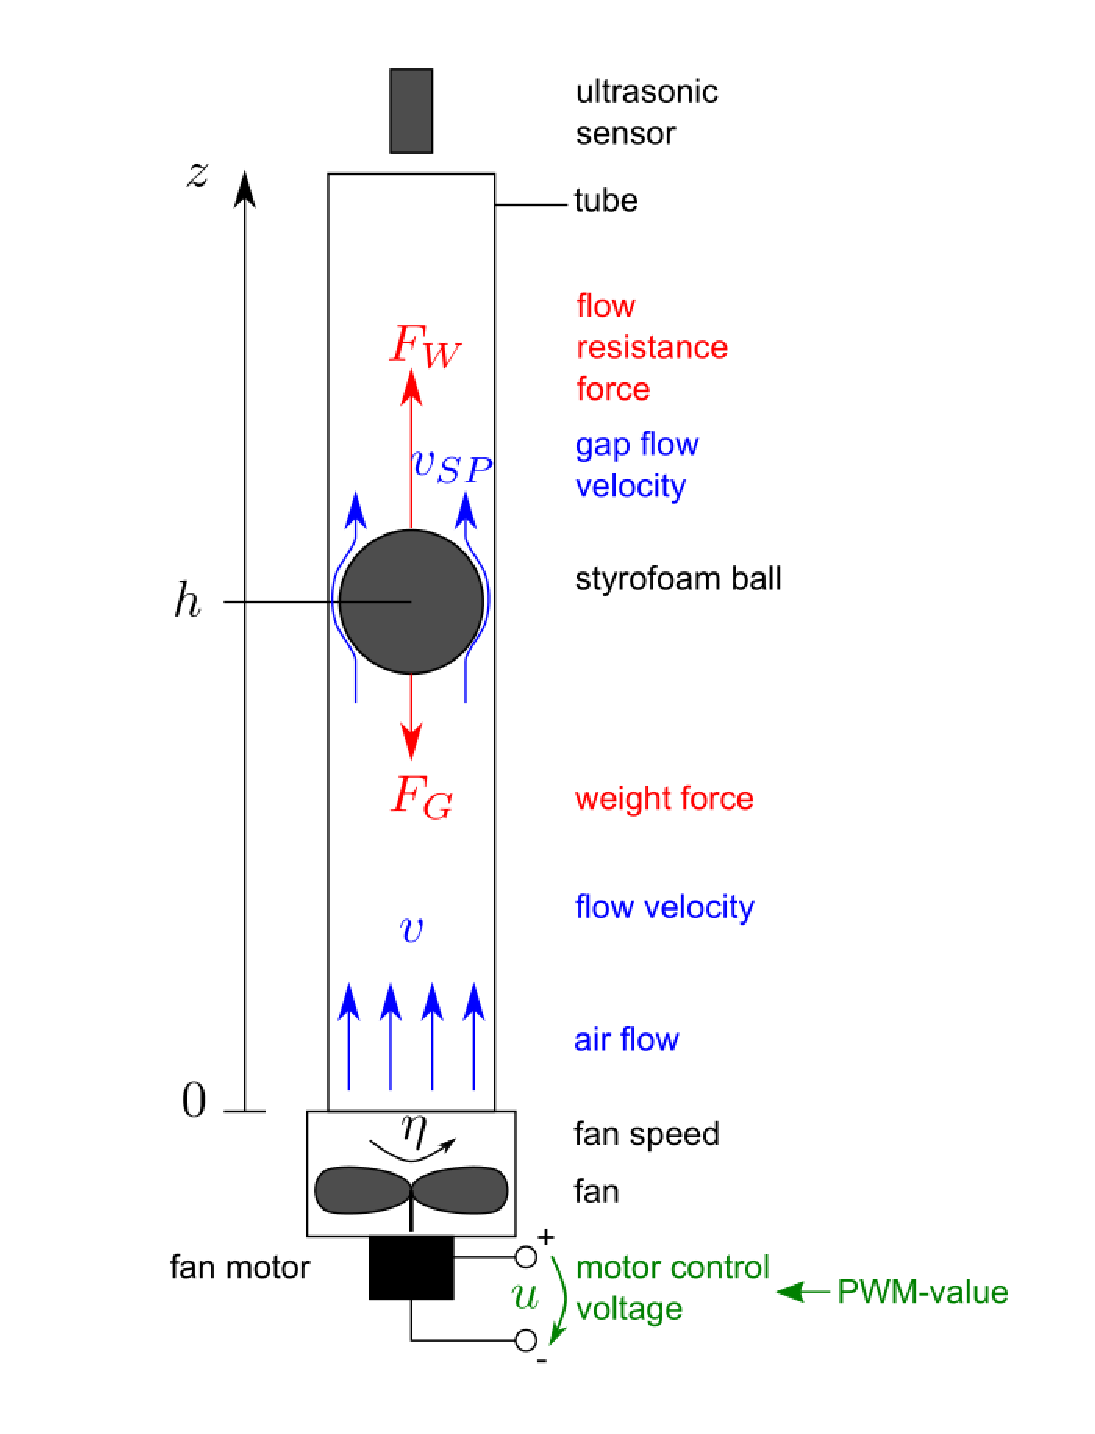
\includegraphics[width=70mm]{ball_in_tube.pdf}
		\caption{Model Structure. \\ \footnotesize{Source: Institut of Control Theory TU Dresden: Regelungstechnikpraktikum, Praktikumsanleitung}}
	\end{figure}

	%%%%%%%%%%%%%%%%%%%%%% MDOEL EQUATIONS %%%%%%%%%%%%%%%%%%%%%%%%%%%

	\section{Model Equations} % MUST

	State Vector and Input Vector:
	\begin{align*}
	    \underline{x} &= (\eta \ h \ \dot{h})^T &= (x_1 \ x_2 \ x_3)^T \\
		\underline{u} &= u_{PWM} &= u \\
	\end{align*}

	\noindent System Equations:
	\begin{subequations}
	\begin{align}
		\dot{x}_1 &= -\frac{1}{T_M}x_1 + \frac{k_M}{T_M}u\\
		\dot{x}_2 &= x_3 \\
		\dot{x}_3 &= \frac{k_L}{m}\left(\frac{k_V(x_1+\eta_0) - A_B\dot{h}}{A_{SP}}\right)^2 -g
	\end{align}
	\end{subequations}

	%%%%%%%%%%%%%%%%%%%%%% PARAMETERS | OUTPUTS %%%%%%%%%%%%%%%%%%%%%%%%%%%
	\noindent
	Parameters: $A_B, \, A_{SP}, \, m, \, g, \, T_M, \, k_M, \, k_V, \, k_L, \, n_0$ % variables with constant, predefined value
	\\
	Outputs: $h$ \\

	%%%%%%%%%%%%%%%%%%%%%% ASSUMPTIONS %%%%%%%%%%%%%%%%%%%%%%%%%%%

	\subsection{Assumptions} % MAY
		\begin{enumerate} %possible list type for the Assumptions
			\item The behavior of the ball does not influence the air flow provided by the fan.
		\end{enumerate}

	%%%%%%%%%%%%%%%%%%%%%% EXEMPLARY PARAMETER VALUES %%%%%%%%%%%%%%%%%%%%%%%%%%%

	\subsection{Exemplary parameter values}
	\begin{tabular}{cl}
\hline
  Symbol  & Value                                                                                                                                                                                \\
\hline
   $A$    & $\left[\begin{matrix}0.8189 & 0.0863 & 0.09 & 0.0813\\0.2524 & 1.0033 & 0.0313 & 0.2004\\-0.0545 & 0.0102 & 0.7901 & -0.258\\-0.1918 & -0.1034 & 0.1602 & 0.8604\end{matrix}\right]$ \\
   $B$    & $\left[\begin{matrix}0.0045 & 0.0044\\0.1001 & 0.01\\0.0003 & -0.0136\\-0.0051 & 0.0936\end{matrix}\right]$                                                                          \\
 $B_{1}$  & $\left[\begin{matrix}0.0045 & 0.0044\\0.1001 & 0.01\\0.0003 & -0.0136\\-0.0051 & 0.0936\end{matrix}\right]$                                                                          \\
 $C_{1}$  & $\left[\begin{matrix}1.0 & 0 & -1.0 & 0\\0 & 0 & 0 & 0\\0 & 0 & 0 & 0\end{matrix}\right]$                                                                                            \\
   $C$    & $\left[\begin{matrix}1.0 & 0 & 0 & 0\\0 & 0 & 1.0 & 0\end{matrix}\right]$                                                                                                            \\
 $D_{11}$ & $\left[\begin{matrix}0 & 0 & 0\\0 & 0 & 0\\0 & 0 & 0\end{matrix}\right]$                                                                                                             \\
 $D_{12}$ & $\left[\begin{matrix}0 & 0\\1.0 & 0\\0 & 1.0\end{matrix}\right]$                                                                                                                     \\
 $D_{21}$ & $\left[\begin{matrix}0 & 1.0 & 0\\0 & 0 & 1.0\end{matrix}\right]$                                                                                                                    \\
\hline
\end{tabular}

	%%%%%%%%%%%%%%%%%%%%%% DERIVATION & EXPLANATION %%%%%%%%%%%%%%%%%%%%%%%%%%%

	\section{Derivation and Explanation} % SHOULD
	The model of the system consists of two submodels. The first one is the model of the ball. Essentially there two forces acting on the ball, the weight force $F_g$ and the force exerted by the flow resistance $F_w$.
	\begin{align}
		F_g &= mg \\
		F_w &= \frac{1}{2} c_w \varrho_L A_B \upsilon_{SP}^2.
	\end{align}
	After inserting the equation for the relative velocity between the sphere and the medium flowing around it $v_{SP}$ and using the proportinal factor $k_V$ we get
	\begin{align}
		F_w &= \frac{1}{2} c_w \varrho_L A_B \left(\frac{k_V(\eta + \eta_0) - A_B \dot{h}}{A_SP}\right)^2.
	\end{align}
	If we now introduce the parameter $k_L$
	\begin{align}
		F_w &= k_L \left(\frac{k_V(\eta +\eta_0) - A_B\dot{h}}{A_SP}\right)^2
	\end{align}
	results.
	Using the vertical force balance, the following equation can be set up.
	\begin{align}
		m\ddot{h}&= k_L \left(\frac{k_V(\eta +\eta_0) - A_B\dot{h}}{A_SP}\right)^2 -mg
	\end{align}
	The second model is the fan. We assume an ordinary fan with pulse width modulation (PWM) control. We are using a model with $PT_1$-behaviour with the time constant $T_M$ an the amplification $k_M$.
	\begin{align}
		T_M \dot{\eta} + \eta = k_Mu_{PWM}
	\end{align}
	%%%%%%%%%%%%%%%%%%%%%% REFERENCES %%%%%%%%%%%%%%%%%%%%%%%%%%%

	\begin{thebibliography}{10}
		\bibitem{But21}Institut of Control Theory TU Dresden:
		\textit{Regelungstechnikpraktikum, Praktikumsanleitung}, published on OPAL April 2022. \\
		(not publicly accessible)

	\end{thebibliography}

\end{document}

